\begin{center}
    \Huge{\textbf{\underline{Exercise 1}}}
\end{center}

\vspace{0.5cm}

Design the class diagram for a flight from the departure airport to the arrival airport.

\vspace{1cm}

\Large{\textbf{\underline{Solution\(_1\)}}}

\begin{center}
    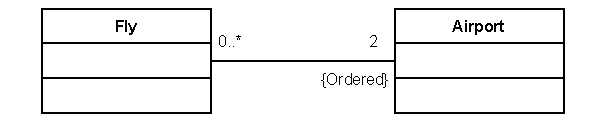
\includegraphics[height=0.12\textheight]{Exercices/EX1/ex1.1.drawio.pdf}
\end{center}

\vspace{0.5cm}

\begin{prettyBox}{Ordered}{myblue}
\{Ordered\} is a constraint applied to a collection of instances where the order of elements
matters.  
For example, in this case, we have a collection of airports where the first element represents
the departure airport, and the second represents the arrival airport.  
\end{prettyBox}

\vspace{1cm}
\Large{\textbf{\underline{Solution\(_2\)}}}

\begin{center}
    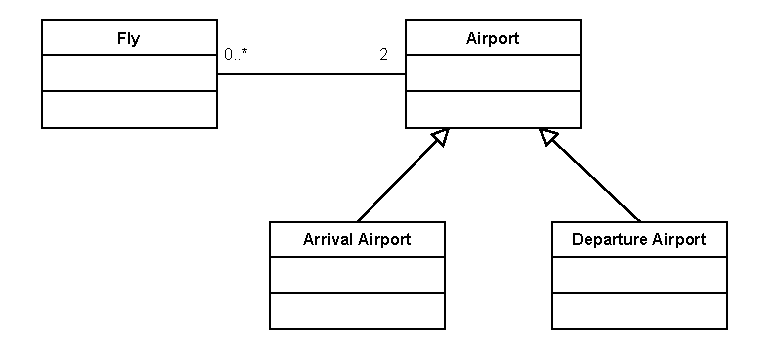
\includegraphics[height=0.3\textheight]{Exercices/EX1/ex1.2.drawio.pdf}
\end{center}

\begin{prettyBox}{Note}{red}
The issue with using inheritance is that it duplicates instances, as each airport would require
a separate instance for departure and another for arrival.  
\end{prettyBox}

\vspace{1cm}
\Large{\textbf{\underline{Solution\(_3\)}}}

\begin{center}
    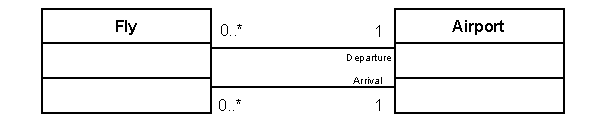
\includegraphics[height=0.12\textheight]{Exercices/EX1/ex1.3.drawio.pdf}
\end{center}

\vspace{0.5cm}

\begin{prettyBox}{Role}{myblue}
A role defines the specific function a class plays in a relationship , a class might have more
than just one role , in our case an airport plays 2 roles : departure or arrival airport.  
\end{prettyBox}

